
\documentclass[../report.tex]{subfiles}
\begin{document}

\graphicspath{{img/}{../img/}}

\subsection{Business Logic Layer Design}

This section will regard implementation of the Business Logic Layer. The design objectives is for the layer to be transparent, supportable, reliable and testable. The rest of the chapter will discus how this was achieved in the implementation. The Supportability and testability goals is traceable to the non-functional requirements NFR-08 and NFR-09.

\paragraph{Overall subsystem design}
Figure \ref{BLLclassdiagram} shows the subsystem structure in the Business Logic Layer(BLL). The Entry factory, BusinessLogicEntryFacoty makes it possible to get hold of the concrete factories without exposing the factories to the service layer. Underneath the Factory lies the Abstract factory pattern which starts with the IBusineesLogicFactory interface. The interface specifies a method for creating each of the abstract products in the abstract factory. The abstract products are IAuthLogic, IUserLogic, IMediaItemLogic, IAccessRightLogic and IDataTransferLogic. The two concrete abstract factory implementations, BusinessLogicFactory and StubFactory, can produce concrete implementation of the abstract products. In this way the service layer can get access to concrete product implementations without exposing them. The abstract products must also implement an internal interface (ie. IAuthInternalLogic) which specifies methods that are used internally in the Business Logic Layer as shown in figure \ref{fig:BusinessLogic_InternalInterfaces} in the appendix. These internal interfaces make it possible for the different concrete logic classes to expose methods to one another but not to the Service Layer. In the BLL implementation all the logic classes use the authentication methods specified in the IAuthInternalLogic interface to authenticate users, admins and clients.

\paragraph{Transparency} \todo{Should this stay?}
In order to gain transparency in the BLL an Abstract Factory pattern with a regular Factory pattern on top has been used (see figure \ref{BLLclassdiagram}). This makes it possible to gain access to the concrete implementations of the Abstract Factory from the Service Layer while only exposing one concrete class, namely the BusinessLogicEntryFactory. The design abstracts interface from concrete implementation and enables the Service Layer using the BLL to only depend on the interface and the factory, but not the concrete implementations.

\paragraph{Supportability} 
The Abstract Factory also achieves supportability. The subsystem is designed to easily support adding new logic
implementations. Adding new factories is not supported in the structure as the developer would have to change the BusinessLogicEntityFactory. The advantage of being able to do so is if different kind of logics supporting different kind of persistence was needed. This is not needed in ShareIT, as the persistence module is dependency injected (allowing persistence to be switched by injecting other persistence implementation), and therefore this structure suffices for the desired level of supportability.

\paragraph{Reliability} \todo{Should this stay?}
Reliability is achieved by having a standard factory on top (EntryFactory). This structure limits the BLL to only having one entry point and therefore being in better control of calls to the subsystem thereby removing the possibility of unsafe operations due to incorrect precedence. 

\paragraph{Testability}
As per the project test strategy every subsystem should be unit and integration tested. Therefore the subsystem is designed to be highly testable through interfacing.

The subsystem also included a test stub. The test stub facilitated ArtShare and SMU clients to be coded up against the logic before it was done. This facilitated parallel development in the project.

\begin{figure}
\centering
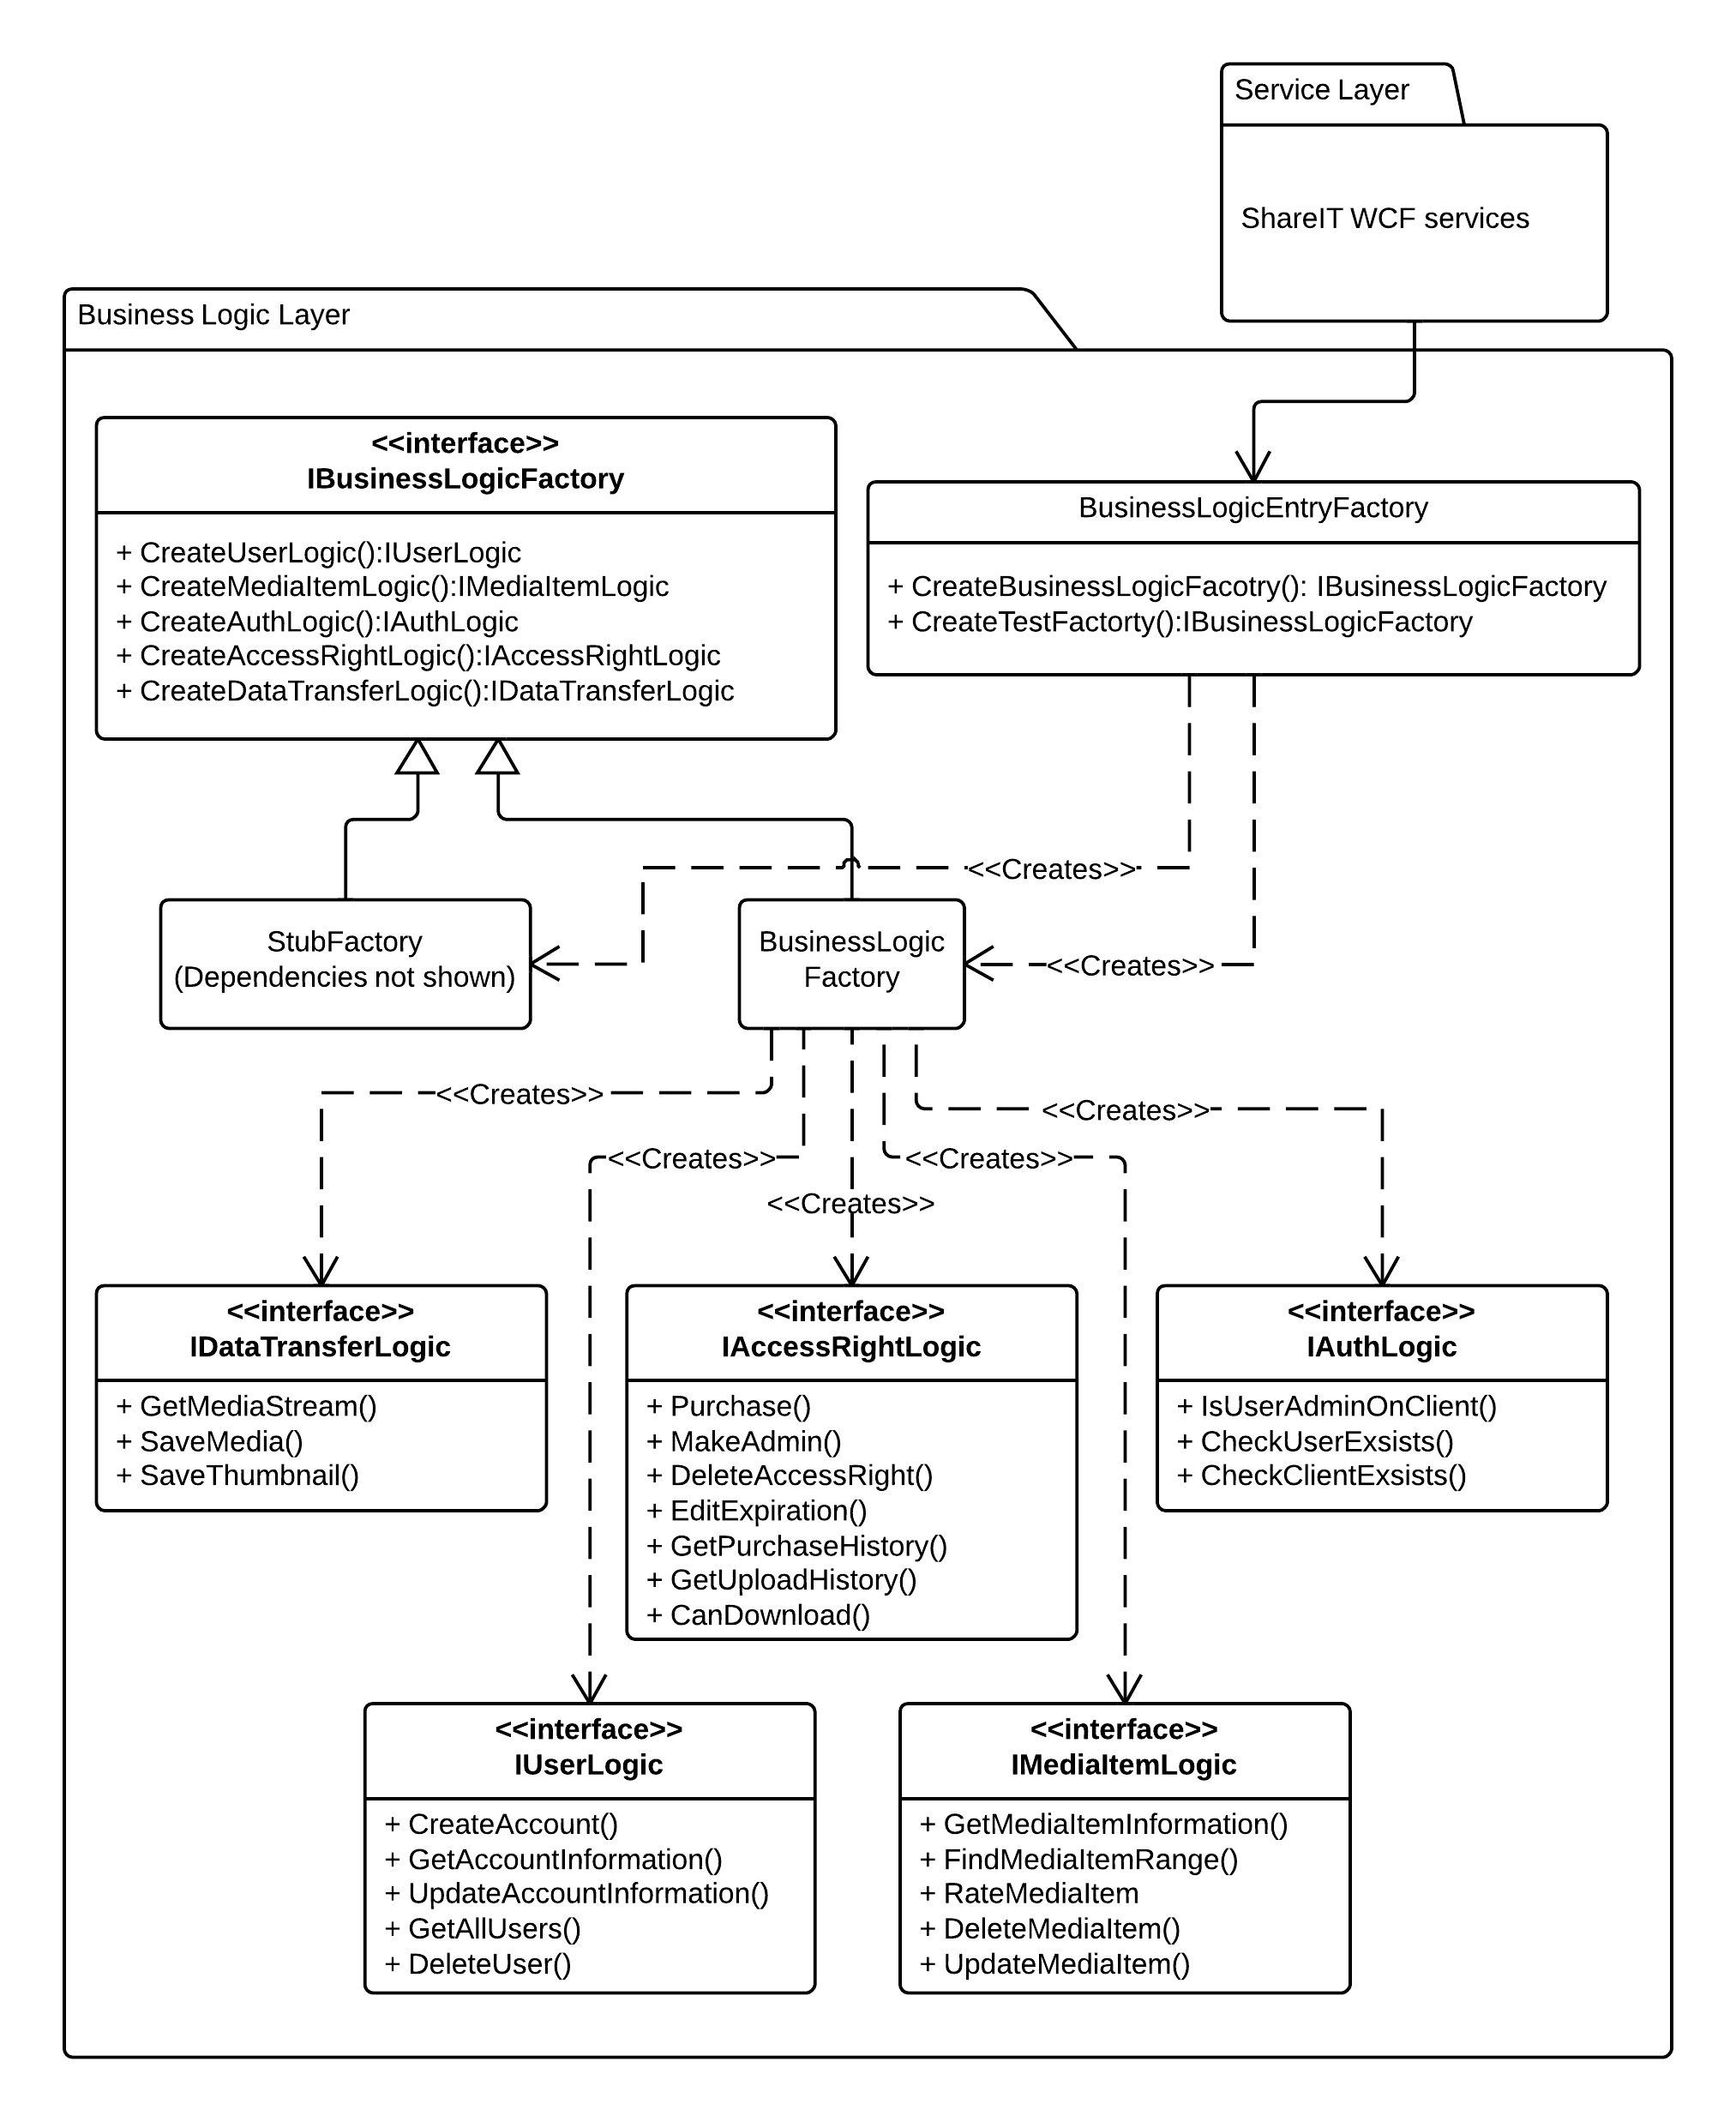
\includegraphics[width=\linewidth]{BLLclassdiagram.png}
\caption{Business Logic Layer class diagram (Not all classes are shown)}
\label{fig:BLLclassdiagram}
\end{figure}




\end{document}